\section{Results}
\label{sec-results}
To evaluate the effectiveness of RSR we will use a generic implementation of A* 
which we run on both original and pruned grid maps.
We discuss performance in terms of \emph{average relative speedup}: 
that is, the improvement to average A* search time and averarage
A* node expansions when running on a pruned  vs. unpruned grid.
Using this metric a search time speedup of 2.0 is twice as fast while
a node expansion speedup of 2.0 indicates half the number of nodes were expanded.
In each case higher is better.
\par
Note that on approximately 2\% of all instances the start and goal are located
in the same rectangle and RSR was able to compute the optimal solution without
search.  We exclude these from our results on the basis that they are outliers,
even though RSR solves these instances in constant time.
\par
First we compare RSR against 4ERR~\cite{harabor10}.  As 4ERR works only on
4-connected grids, here we restrict our attention to this type of maps.  To
assess the invidual impact of both perimeter reduction (PR) and online node
pruning (OP) we also develop and compare two variant algorithms: 4ERR+PR and
4ERR+OP.

Next, we compare and contrast the performance of RSR with the Swamps
algorithm~\cite{pochter10}.  Here we use the 8-connected variants of each
benchmark, both in their original size and scaled by a factor of 3.  When
evaluating Swamps we used the authors' source code and ran all experiments using
their recommended running parameters: a swamp seed radius of 6 and ``no change
limit'' of 2.
\par 
\begin{figure*}[t]
       \begin{center}
                       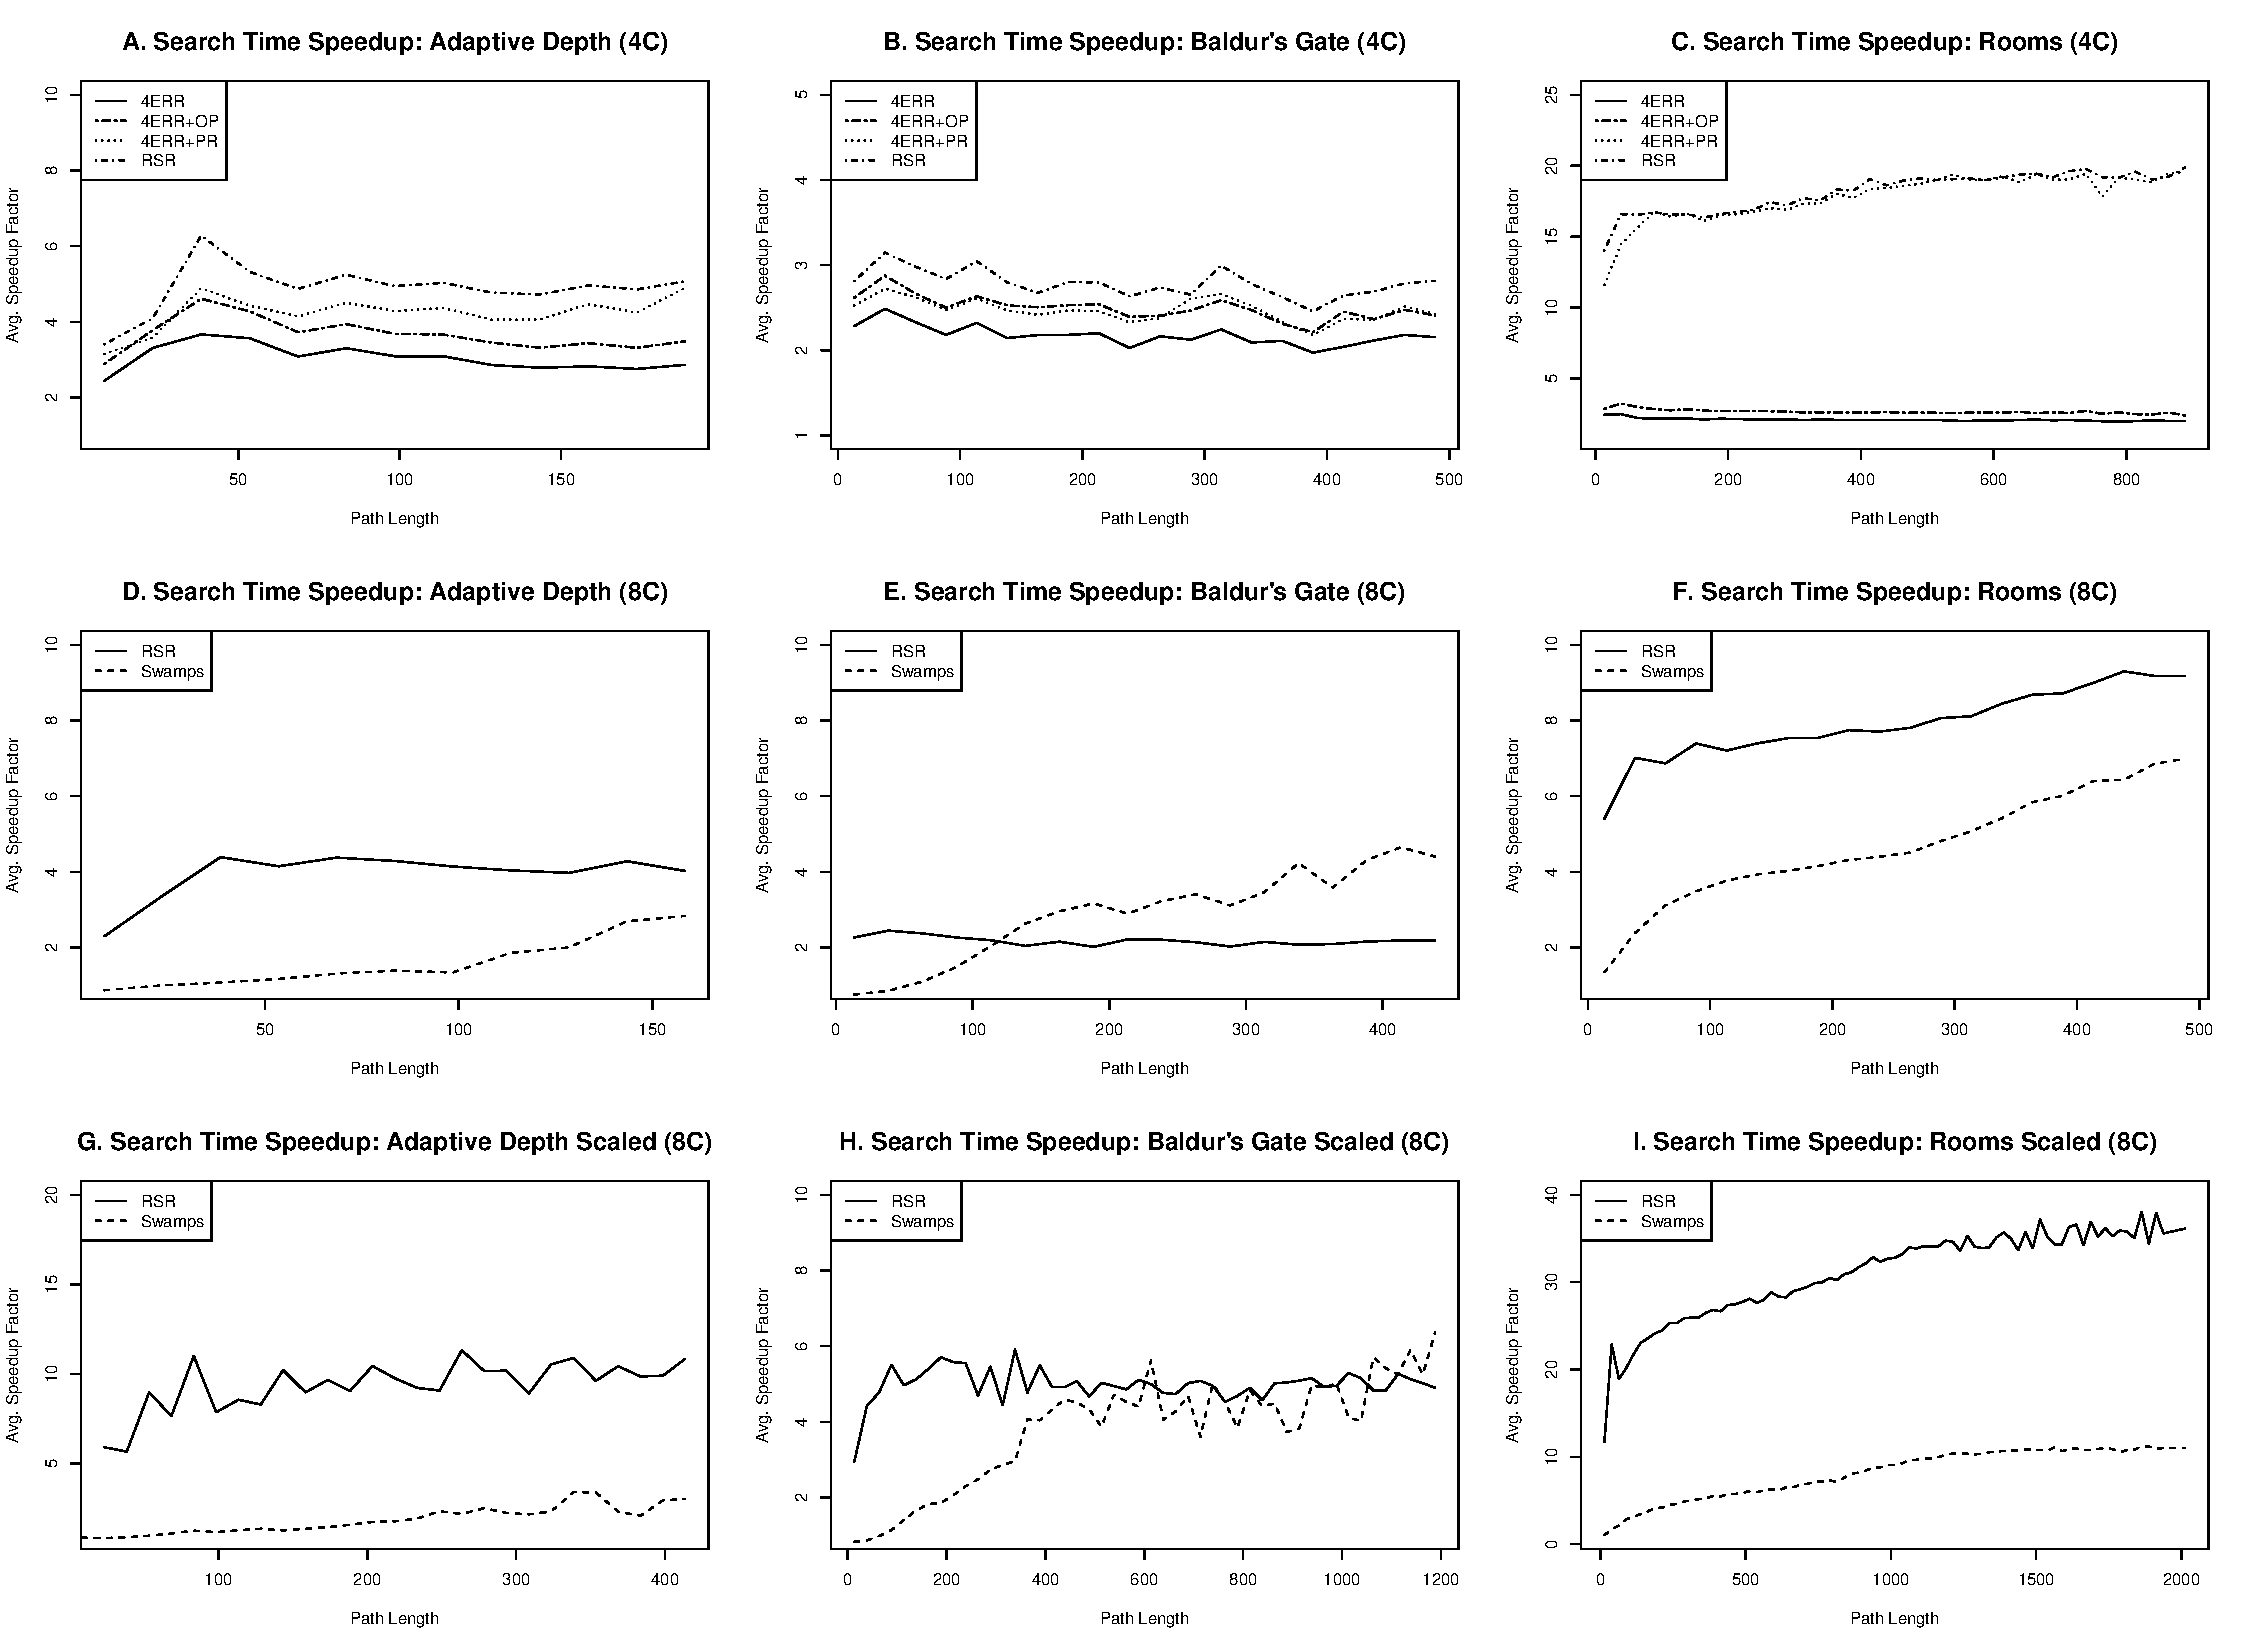
\includegraphics[width=1.85\columnwidth, trim = 10mm 10mm 10mm 0mm]{diagrams/speedup.pdf}
       \end{center}
       \caption{Average A* speedup on each of our three benchmarks. 
		Results are given in terms of search time.}
\label{fig-speedup}
\end{figure*}

\par
\textbf{Comparison with 4ERR and Impact of PR and OP:}
As per Figure \ref{fig-speedup} (A to C), we note that RSR shows a convincing 
speed-up improvement over 4ERR and all its variants across all input maps.
This allows us to conclude that that RSR is the better choice on 4-connected maps.
\par
When analysing the impact of each enhancement, we note that 4ERR+PR yielded the
biggest improvement on all three benchmarks.
The most dramatic example can be seen on Rooms (Figure \ref{fig-speedup}C) 
where 4ERR+PR speeds up A* by 20 times.
Meanwhile, 4ERR+OP compares well with PR on both Adaptive Depth and
Baldur's Gate but is of little benefit on Rooms.
%In an additional experiment, we evaluated the impact of OP on 8-connected
%grids and observed that its contribution to speedup was more significant than in 
%the 4-connected case.
%This can be explained as follows: on 4-connected maps, 4ERR maintains a very low
%branching factor, which is comparable (and even slightly better) than the branching
%factor on the original map. 
%On the other hand, 8ERR (i.e. RSR without OP and PR speedup enhancements) 
%can introduce larger branching factors. Therefore, there are more opportunities for 
%online pruning in the latter case. 
%Other details (and charts) are left out because of rectangle limitations.
\par
Finally, it is interesting to note the sometimes large performance variation 
from one benchmark to another. This is indicative of how effectively we can 
decompose the different maps into rectangular shaped regions.
For example, the maps in the Rooms set are highly suited to this approach but those
from Baldur's Gate, which have an unusual 45-degree orientation, are not.
\par
\textbf{Comparison to Swamps:}
Figure \ref{fig-speedup} (D to F) gives search time speedup results for both RSR
and Swamps running on the 8-connected variants of our three benchmark problem
sets. On this subset of input data, the results are mixed.
On Adaptive Depth and Rooms, RSR achieves higher
speedups and is shown consistently better than Swamps. However, on Baldur's
Gate, this trend is reversed.  
It is interesting to note that on the
benchmarks where RSR performs well there are usually large open areas and the
terrain can often be naturally decomposed into rectangles.  This is not
true for the Baldur's Gate benchmark where Swamps-based pruning appears to be
more effective.
\par
To test this hypothesis we scaled each map in every benchmark by a factor of 3
and generated a new set of 100 problem instances per map. 
Scaling has the effect of producing larger open areas and allows 
us to measure the impact of this variable on search time speedup.
We present our findings in  Figure \ref{fig-speedup} (G to I).
We observe that while the maximum speedup achieved by both algorithms has
increased, the gain for Swamps is very small while RSR shows dramatic
improvement.
Infact, if we limit our attention to problems of similar length to those seen 
on the original maps we notice that the performance of Swamps actually
decreases.
\par
The observed performance characteristics are not unexpected: Swamps prune out
areas that can be avoided without introducing a detour while rectangle-based
symmetry reduction allows for a faster exploration of areas that need to be
searched.  Since it appears that the two algorithms are orthogonal, a natural
extension of this work would be to combine the two: first, apply 4(or 8)ERR+PR
(as appropriate) to a grid in order to eliminate as many interior nodes as
possible; then, apply a Swamps-based decomposition to the resultant graph.
